

% ========================================
%
% ========================================
\section{\acp{FSM} modelling in \SV}
\begin{frame}{FSMs modeling in SystemVerilog}{}
\begin{itemize}
  \item \typedef may be used in order to define the states of the \ac{FSM}.
  \begin{itemize}
    \item[] \code{\typedef \enum \{IDLE, LOAD, PROCESS, STORE\} state\_t;}
    \item[] \code{state\_t current\_state;}
    \item[] \code{state\_t next\_state;}
  \end{itemize}
  \item Two main approaches for modelling \acp{FSM} in \SV.
  \begin{itemize}
    \item Separate combinational logic (next state and output logic) from state registers.
    \item One single process for both combinational logic and state registers.
  \end{itemize}
\end{itemize}
\end{frame}


%% ========================================
%%
%% ========================================
%\begin{frame}{}{}
%\begin{figure}
%  \centering
%  \begin{subfigure}{\textwidth}
%    \centering
%     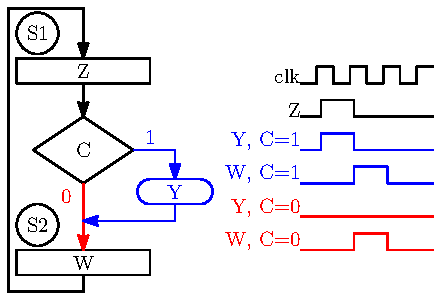
\includegraphics[scale=0.7]{ASM_chart_conditional}
%     \caption{Conditional output.}
%     \label{Figure:ASM_conditional}
%  \end{subfigure}
%  \\
%  \begin{subfigure}{\textwidth}
%    \centering
%    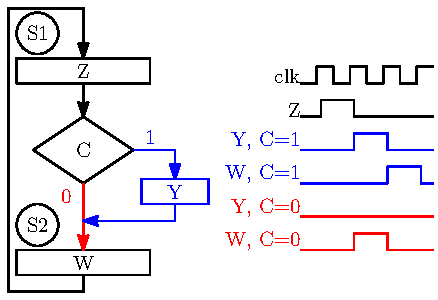
\includegraphics[scale=0.7]{ASM_chart_unconditional}
%    \caption{Unconditional output.}
%    \label{Figure:ASM_unconditional}
%  \end{subfigure}
%  \vspace{-12pt}
%  \caption{Conditional and unconditional outputs}
%  \label{Figure:ASM_outputs}
%\end{figure}
%\end{frame}
%
%
\section{Testbenches}
% ========================================
%
% ========================================
\begin{frame}{Testbenches}{}
\begin{itemize}
\item Testbenches are \alertblue{non-synthesizable} modules that verify the correct functionality of our designs.
\item They consist of test vectors, simply referred to as \alertblue{stimulus}, that are input into the \ac{DUT}.
\item Testbenches are also in charge of verifying the response of the \ac{DUT}.
\end{itemize}
\end{frame}

% ========================================
%
% ========================================
\begin{frame}{Testbenches}{}
  \begin{figure}
    \centering
    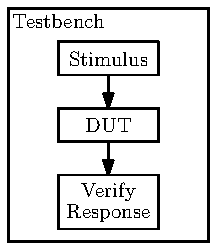
\includegraphics[scale=1.7]{testbench_diagram}
    \vspace{-2pt}
    \caption{Block diagram of a testbench.}
    \label{Figure:Testbench_diagram}
  \end{figure}
\end{frame}

% ========================================
%
% ========================================
\begin{frame}{Testbenches}{}
\begin{itemize}
\item Characteristics of testbenches.
\begin{itemize}
\item Non-synthesizable.
\item No \ac{IO} ports.
\item \ac{DUT}'s \ac{IO} ports are accessed through local signals.
\item Support the full scope of \SV language, \ie, delays, system calls, initial blocks, assertions, reading/writing from/to files, \emph{etc.}.
\end{itemize}
\item They consist of test vectors, simply referred to as \alertblue{stimulus}, that are input into the \ac{DUT}.
\item Testbenches are also in charge of verifying the response of the \ac{DUT}.
\end{itemize}
\end{frame}

% ========================================
%
% ========================================
\begin{frame}{Basic structure of a testbench}{}
\begin{itemize}
\item Generally speaking, a testbench is composed of the following parts.
\begin{enumerate}
\item Module declaration (no \ac{IO} ports).
\item \ac{IO} ports from \ac{DUT} are accessed through internal signals.
\item \ac{DUT} instantiation.
\item Stimuli generation.
\item Response checker.
\end{enumerate}
\end{itemize}
\end{frame}

% ========================================
%
% ========================================
\begin{frame}{Basic structure of a testbench}{}
\begin{itemize}
\item Module declaration.
\lstset{numbers=none, xleftmargin=.1\textwidth, xrightmargin=.1\textwidth}
\begin{lstlisting}
module testbench;
    // testbench code
endmodule:testbench;
\end{lstlisting}
\end{itemize}
\end{frame}

% ========================================
%
% ========================================
\begin{frame}{}{}
\begin{itemize}
\item \ac{IO} ports from \ac{DUT} are accessed through internal signals.
\end{itemize}
   \vspace{-5pt}
\begin{figure}
  \centering
  \begin{subfigure}{\textwidth}
    \centering
     \includegraphics[scale=0.5]{testbench_dut_ports}
     \caption{\ac{DUT}'s \ac{IO} ports.}
     \label{Figure:DUT_IO_ports}
  \end{subfigure}
  \\
 \vspace{-5pt}
  \begin{subfigure}{\textwidth}
    \centering
    \includegraphics[scale=0.5]{testbench_dut_internal}
    \caption{Testbench internal signals.}
    \label{Figure:Testbench_internal_signals}
  \end{subfigure}
  \vspace{-12pt}
  \caption{Accessing \ac{DUT}'s \ac{IO} port in testbenches}
  \label{Figure:DUT_IOs}
\end{figure}
\end{frame}

% ========================================
%
% ========================================
\begin{frame}{Basic structure of a testbench}{}
\alertblue{\ac{DUT} instantiation.}
\begin{itemize}
\item \ac{DUT} instantiation.
\end{itemize}
  \begin{figure}
    \centering
    \includegraphics[scale=0.8]{testbench_dut_instantiation}
    \vspace{-2pt}
    \caption{\ac{DUT} instantiation.}
    \label{Figure:DUT_instantiation}
  \end{figure}
\end{frame}

% ========================================
%
% ========================================
\begin{frame}{Basic structure of a testbench}{}
\begin{itemize}
\item Here, the convention used is.
\item[] \code{\textcolor{blue}{design\_name}}
\item[] \code{\textcolor{red}{dut\_instance\_name}(.\textcolor{blue}{design\_IO\_port\_1}(\textcolor{red}{testbench\_signal\_1}),}
\item[] \code{~~~~~~~~~~~~~~~~~.\textcolor{blue}{design\_IO\_port\_2}(\textcolor{red}{testbench\_signal\_2}),}
\item[] \code{~~~~~~~~~~~~~~~~~.\textcolor{blue}{design\_IO\_port\_3}(\textcolor{red}{testbench\_signal\_3}),}
\item[] \code{~~~~~~~~~~~~~~~~~$\vdots$}
\item[] \code{~~~~~~~~~~~~~~~~~.\textcolor{blue}{design\_IO\_port\_n}(\textcolor{red}{testbench\_signal\_n})}
\item[] \code{~~~~~~~~~~~~~~~~~);}
\end{itemize}
\end{frame}


% ========================================
%
% ========================================
\begin{frame}{Basic structure of a testbench}{}
\begin{itemize}
\item Alternatively, \SV supports instantiation using the \emph{dot-star} notation.
\item[] \code{\textcolor{blue}{design\_name} \textcolor{red}{dut\_instance\_name}(.*);}
\item This notation will automatically connect all \ac{IO} ports from the design to the internal signals from the testbench.
\item This will only occur \alertred{IF ALL} \ac{IO} ports from the design and the internal signals from the testbench have the same name.
\end{itemize}
\end{frame}

% ========================================
%
% ========================================
\begin{frame}{Basic structure of a testbench}{}
\begin{itemize}
\item Stimuli generation.
\begin{itemize}
\item Stressing \alertblue{input} ports from design.
\item A combination of input vectors is known as a test case.
\item Several test cases must be applied in order to verify the design's correctness.
\item Test cases may be provided via input files, in which case, the expected output is also provided as a reference.
\item Delays are paramount in generating and driving test vectors into the \ac{DUT}.
\item Delays provide \acp{DUT} enough time to react to the stimuli in order to generate their outputs.
\end{itemize}
\end{itemize}
\end{frame}

% ========================================
%
% ========================================
\begin{frame}{Basic structure of a testbench}{}
\alertblue{Delay generation.}
\begin{itemize}
\item \SV provides different ways of delay generation.
\begin{itemize}
\item Specifying the exact amount and time units.
\begin{itemize}
\item[] \code{\#10ns;}
\item[] \code{\#200us;}
\item[] \code{\#50ps;}
\end{itemize}
\pauseprint
\item Via reference to simulation's timescale at the beginning of the testbench code.
\begin{itemize}
\item[] \code{\textcolor{blue}{`timescale} unit/precision}
\end{itemize}
\pauseprint
\item For example.
\begin{itemize}
\item[] \code{\textcolor{blue}{`timescale} 1ns/10ps}
\end{itemize}
\item After this, we can generate delays by simply having
\begin{itemize}
\item[] \code{\#3}
\end{itemize}
\item This will generate a delay of 3 time units, \ie, 3ns.
\item The smallest delay we could generate in this example is \code{\#0.01} \ie, 10ps.
\begin{itemize}
\item[] \code{\#0.7} and \code{\#0.07} will generate delays of 700ps and 70ps, respectively
\end{itemize}
\end{itemize}
\end{itemize}
\end{frame}

% ========================================
%
% ========================================
\begin{frame}{Basic structure of a testbench}{}
\begin{itemize}
\item Generate a clock signal with a period of 10ns.
\pauseprint
\item[] \code{\textcolor{blue}{always begin}}
\item[] \code{~~clk = 1'b0;}
\item[] \code{~~\#5ns; // \#5 if time unit is 1ns}
\item[] \code{~~clk = 1'b1;}
\item[] \code{~~\#5ns; // \#5 if time unit is 1ns}
\item[] \code{\textcolor{blue}{end}}
\end{itemize}
\end{frame}


% ========================================
%
% ========================================
\begin{frame}{Basic structure of a testbench}{}
\alertblue{Clocking blocks.}
\begin{itemize}
\item Once a clock signal is generated, we can generate delays in terms of clock cycles instead of time units.
\item In order to do this, we must first declare a \codeblue{default clocking} block.
\item[] \codeblue{default clocking} \code{clock @(}\codeblue{posedge}\code{ clk);}
\item[] \codeblue{endclocking}
\item \code{\#\#1 // Will generate a delay of 1 clock cycle.}
\item \code{\#\#37 // Will generate a delay of 37 clock cycles.}
\end{itemize}
\end{frame}


% ========================================
%
% ========================================
\begin{frame}{Basic structure of a testbench}{}
\begin{itemize}
\item \codeblue{initial} blocks are used in testbenches in order to execute procedures only once.
\item A common misconception is that the name \codeblue{initial} refers to initialisation.
\item They are commonly used to drive reset signals.
\item \codeblue{initial} blocks should not be used for synthesis.
\item[] \codeblue{initial begin}
\item[] \code{~~reset = 0;}
\item[] \code{~~\#\#2;}
\item[] \code{~~reset = 1;}
\item[] \code{~~\#\#3;}
\item[] \code{~~reset = 0;}
\item[] \codeblue{end }
\end{itemize}
\end{frame}

% ========================================
%
% ========================================
\begin{frame}{Basic structure of a testbench}{}
\begin{itemize}
\item It is a good practice to avoid driving signals exactly at the clock edge.
\item This may lead to confusion relating to in which clock edge data is being sampled.
\item It is a good practice to add a small delay in the signals that drive data into our \ac{DUT}.
\item This is useful in order to emulate propagation delays of logic gates.
\end{itemize}
\end{frame}

% ========================================
%
% ========================================
\begin{frame}{Basic structure of a testbench}{}
  \begin{figure}
    \centering
    \includegraphics[scale=0.49]{testbench_input_delay_sv}
    \vspace{-6pt}
    \caption{Generating input delays in testbenches.}
    \label{Figure:testbench_input_delay_sv}
  \end{figure}
\end{frame}


% ========================================
%
% ========================================
\begin{frame}{Basic structure of a testbench}{}
  \begin{figure}
    \centering
    \includegraphics[width=\textwidth]{testbench_input_delay_wave}
    \vspace{-8pt}
    \caption{Input delays in waveforms.}
    \label{Figure:testbench_input_delay_wave}
  \end{figure}
\end{frame}
